% tools voor document
\documentclass{article} % definieer type document (article, resume, etc...)
\usepackage[english]{babel} % definieer taal van document
\usepackage{graphicx}
\usepackage[a4paper]{geometry} % definieer formaat van document
\usepackage{hyperref}

\begin{document}
    %%%%%% TITLE PAGE %%%%%
    \sffamily
    \begin{titlepage}
        \centering
        \vfill
        {\bfseries\Huge
            TINLAB Machine Learning \\
            \vskip1cm
        }
        {\bfseries\Large
            TINLML02 \\
            \vskip4cm
        }
        {\bfseries\Huge
            Persoonlijk verslag \\
            \vskip1cm
        }
        {\bfseries\Large
            Thijs Dregmans\\
        }
        {\bfseries\normalsize
            1024272@hr.nl\\
            \vskip1cm
            \today\\
        }    
        \vfill
        % \includegraphics[width=4cm]{frontpage_image.png}
        \vfill
        \vfill
    \end{titlepage}
    \newpage

    %%%%% TABLE OF CONTENTS %%%%%
    \tableofcontents
    \newpage

    %%%% INTRO %%%%
    \section*{Introductie}

    Voor mijn opleiding Technische Informatica was er de mogelijkheid te kiezen voor Machine Learing. Mijn keuze voor ML was heel bewust. \\
    Iedereen praat over AI maar niemand weet precies hoe het werkt. (Dat is het beeld bij mij.) Het zelf bouwen en trainen van een neuraal netwerk lijkt me leuk en heel leerzaam. Ook de discussie over de filosofische en ethische aspecten zijn heel interessant. De invloed van je mensbeeld op beeldvorming van AI en/of machine learning is enorm. Het lijkt me leuk om deel te nemen aan die discussie. \\ \\
    In dit verslag beschrijf ik welke kennis ik tijdens de cursus heb verworven, welke opdrachten ik heb gemaakt, hoe ik daarbij te werk ben gegaan en ik reflecteer op het project en de leerdoelen.

    \newpage

    %%%%% Verworven kennis en persoonlijke opdrachten voortgang %%%%%
    \section{Verworven kennis en persoonlijke opdrachten voortgang}

        De cursus is opgedeeld in 2 persoonlijke programmeer opdrachten en 1 groepsopdracht. \\
        De broncode voor elke opdracht is te vinden op de Github pagina: \href{https://github.com/tdregmans/TINLML02-persoonlijk-verslag}{tdregmans/TINLML02-persoonlijk-verslag} De verschillende branches bevatten verschillende versies van de opdrachten.

        %%%%% NEURALE NETWERKEN %%%%%
        \subsection{Opdracht 1: Neurale Netwerken}
        
            In de eerste opdracht is het doel om te gaan begrijpen hoe een Neuraal Netwerk in elkaar zit. \\
            \begin{center}
                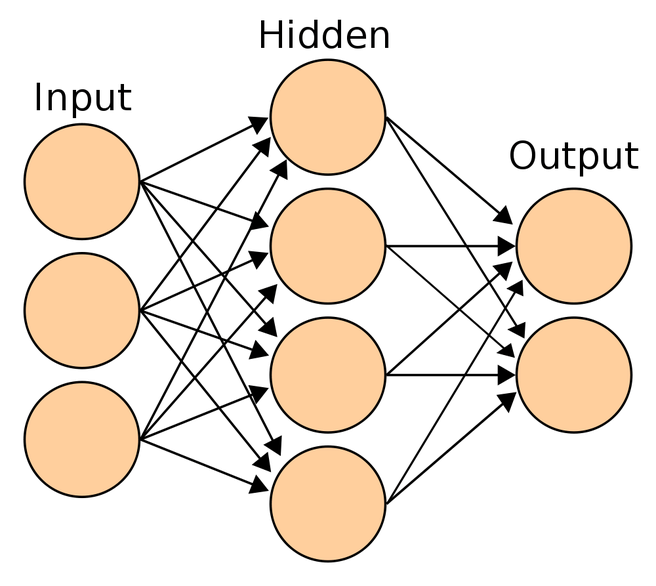
\includegraphics[width=7cm]{nn.png}
            \end{center} 
            
            Een Neuraal Netwerk bestaat uit zogenaamde 'nodes' en 'links'. De 'nodes' zijn de knoppen in het netwerk en de 'links' zijn de pijlen die tussen de nodes lopen, in elke laag. \\
            In het voorbeeld hierboven zijn er 3 lagen: 1 input laag, 1 'hidden' laag en 1 output laag. \\
            De input nodes zijn de parameters. Die krijgen een bepaalde waarde. De links geven die vervolgens door aan de nodes in de volgende laag. Die nodes hebben weer links naar de output laag. De links geven de waardes door aan die laag. De links geven de waade niet zomaar door. Elke link heeft een gewicht. Dat is een getal waarmee de waarde van de node mee wordt vermenigvuldigd. Door de gewichten te varieren tellen bepaalde nodes (die inputs voorstellen) zwaarder dan anderen. Dit zorgt voor het 'slimme' van het netwerk. \\ \\
            Voor deze opdracht moest een Neuraal Netwerk gebouwd worden in Python waarmee een cirkel van een kruis onscheiden moest kunnen worden. De symbolen werden voorgesteld door een serie van 3x3 bits. \\
            Voor de eerste versie van de opdracht is begonnen met het implementeren van de intuitieve classes 'Node', 'Link' en 'NeuralNetwork'. Dit komt overeen met \href{https://github.com/tdregmans/TINLML02-persoonlijk-verslag/tree/opdracht1-v2.0/opdracht1}{branch opdracht1-v2.0}. \\ \\
            Na gebruik van 'Node' en 'Link' objecten is overgegaan op gebruik van numpy matrices om de gewichten te bewaren. Dit heeft als voordeel dat het sneller is, en een kleinere codebase vereist. Dit is geimplementeerd in \href{https://github.com/tdregmans/TINLML02-persoonlijk-verslag/tree/opdracht1-v3.1/opdracht1}{branch opdracht1-v3.1}. \\ \\
            Alle versies t/m \(v4.*\) veranderen de gewichten random. Er wordt dan gekeken of de verandering tot een beter resultaat heeft geleid. Als dat niet zo is, dan wordt de verandering teruggedraaid. Mocht dat wel zo zijn, dan is het model verbeterd in die cycli. De verandering blijft dan staan. Vanaf versie \(v5.0\) wordt gebruik gemaakt van een Neuraal Netwerk dat met behulp van een 'cost-function' en backward propagation efficient het model verbeterd. Dit is gebaseerd op een code-snippet van geeksforgeeks.com: \href{https://www.geeksforgeeks.org/backpropagation-in-machine-learning/#example-of-backpropagation-in-machine-learning}{example of backpropagation in machine learning}. Dit voorbeeld is aangepast zodat het toepasbaar voor deze opdracht. Het is geimplementeerd in \href{https://github.com/tdregmans/TINLML02-persoonlijk-verslag/tree/opdracht1-v5.0/opdracht1}{branch opdracht1-v5.0}.
    
        \newpage

        %%%%% GENETISCHE ALGORITMEN %%%%%
        \subsection{Opdracht 2: Genetische Algoritmen}
        
            In de tweede opdracht wordt een uitstapje gemaakt naar Genetische Algoritmen. Een Genetische Algoritme is een algoritme dat natuurlijke selectie gebruikt, om tot betere resultaten te komen. Net als in de natuur, wordt door natuurlijke selectie geselecteerd op een bepaalde kwaliteit. Dit resulteert in het meer voorkomen van die kwaliteit. \\
            Er wordt begonnen met een intiële populatie. Op deze populatie wordt een random mutatie toegepast. Vervolgens wordt volgens de fitheid van deze nieuwe generatie bepaalt. In de opdracht is dit een score gegeven door de gebruiker. Er is gekozen voor een rating van 0 t/m 10 die de gebruiker aan de muziek kan geven. \\
            In deze opdracht is de intiële populatie muziek van Bach, zoals aangeleverd door de docenten. Op deze muziek worden random mutatie toegepast. Op basis van de rating van de gebruiker, wordt de muziek vervolgens aangepast. \\
            Er is in deze implementatie gekozen om telkens de beste muziek die daarvoor gegenereerd is, te gebruiken voor de nieuwe generatie. Wat de 'beste' muziek is, is bepaald door de gebruiker. \\
            De architectuur van de software is soortgelijk aan die van opdracht 1: Er is een 'main.py' die het programma aanstuurt. Deze importeert de 'Generator' klasse, en maakt hier een object van. Die wordt vervolgens gebruikt om muziek te genereren. Op de achtergrond wordt gebruik gemaakt van de 'muser.py' die door het docententeam geleverd is. \\
            Er is een simpele implementatie te vinden in  \href{https://github.com/tdregmans/TINLML02-persoonlijk-verslag/tree/opdracht2-v1.0/opdracht2}{branch opdracht2-v1.0}.
    
        \newpage

        %%%%% TORCS %%%%%
        \subsection{Eindopdracht: TORCS Neuraal Netwerk}
        
            Voor de eindopdracht was het de bedoeling om een model te maken dat een auto kan besturen. In de TORCS simulatie kreeg elke groep een auto. Vervolgens gaan alle auto's tegen elkaar racen. De auto die het parcours het snelst aflegt, wint. De inhoudelijke uitwerking van onze groep is te vinden in de opleverset en de \href{https://github.com/tdregmans/TINLML02}{GitHub repository tdregmans/TINLML02}. \\
            De opdracht was heel leuk om te doen. Ik heb er veel van geleerd. Uiteindelijk is het onze groep ook gelukt om een werkende auto te maken, maar dat heeft wel veel moeite gekost. Lang niet alle lessen waren relevant en/of duidelijk. We hebben veel zelf moeten uitzoeken, maar daar leer je wel het meest van. 
    
        \newpage

    %%%%% Persoonlijke evaluatie op project en leerdoelen %%%%%

    \section{Persoonlijke evaluatie op project en leerdoelen}

    De leerdoelen voor deze cursus lijken veel op de doelen voor de stage. We hebben de eindopdracht ook zo aangepakt; in lijn met de projectdoelen. We hebben eerst requirements opgesteld. Daarna hebben we ontwerpen gemaakt. Deze hebben we uitgewerkt. Noodzakelijke kennis hebben we verkregen door onderzoek te doen. Het prototype is uiteindelijk iets dat werkt. Dit hebben we geverifeerd middels tests, die gebaseerd zijn op de requirements. Na aanleiding van het project hebben we aanbevelingen gedaan. \\
    Ik vond het een leerzaam vak. Voordat ik aan het vak begon, wist ik heel weinig van de werking van AI. Nu heb ik van dichtbij gezien hoe het werkt. Ik heb zelf een AI geïmplementeerd en getest. Samen met het team, hebben we een AI kunnen maken die een race auto bestuurt. Dat is zeker een mooi resultaat. Ook de ethische discussies vond ik mooi. Met de boekenclub heb ik veel lol gehad. Ik heb met andere studenten van gedachten gewisseld. Dat was zeker waardevol. \\
    Ik ben tevreden met wat ik heb geleerd. Ik had inhoudelijk iets meer van de lessen verwacht, maar al met al ben ik tevreden met het resultaat en de geleerde vaardigheden.

    \newpage


\end{document}
